%% International Journal of Computational Intelligence Systems ---
%%%%%%%%%%%%%%%%%%%%%%%%%%%%%%%%%%%%%%%%%%%%%%%%%%%%%%%%%%%%%%%%%%%%%%%%%%%
\documentclass[11pt,twoside]{article}
\usepackage{ap-article}
%--------------------- ADDITIONAL PACKAGES HERE ---------------------------
% Authors shoud add additional packages here. 
% For example, PsTricks and/et pst-* for drawing that use the 
% command latex+dvips+ps2pdf 
% or TikZ for commands pdflatex ...
%--------------------------------------------------------------------------
%
\def\labart{yourLabel}      % put a label from your choice here
%\Vol{1}                    % number of the Volume
%\Issue{1}                  % number of the issue
%\Month{January}            % month
%\Year{2008}                % year
%\received{...}
%\revised{...}
%
%---------------------------------------------------------------------------
\thispagestyle{empty}
%%------------------------- YOUR HEADINGS HERE -----------------------------
% Author's initials of first names+last names
\shortauthors{Author's Names}
% Short title
\shorttitle{Paper Title (4 Words maximum)}
%---------------------------------------------------------------------------
%
%---------------------- YOUR TITLE ----------------------------------------
\title{%
Instructions for Typesetting Manuscript \\ \vspace*{0.04truein}
Using \LaTeX\footnote{For the title, try not to use more than 3 lines. Typeset the title in 12 pt Times Roman, boldface.}
}
%-------------------------- AUTHOR'S NAMES ----------------------------------
\author{%
First Author\,\up{1}\,\footnote{Typeset names in 10 pt Times Roman, boldface. Use the footnote to indicate the present or permanent address of the author.}\,,\
Second Author\,\up{2}
}
%----------------------------- ADDRESSES ----------------------------------
\addresses\address{%
\\ \vspace*{0.05truein}
\up{2}
Group, Company,\\
Address,\\ City, State ZIP/Zone, Country \\ 
\vspace*{0.04truein}
E-mail: address
}
%---------------------------------------------------------------------------
\pagestyle{myheadings}
\begin{document}
\label{\labart-FirstPage}

\maketitle
%-------------------------- ABSTRACT ---------------------------------------
\abstracts{%
The abstract should summarize the context, content and conclusions of the paper in less than 80 words. It should not contain any references or displayed equations. Typeset the abstract in 9~pt Times Roman with baselineskip of 11 pt, making an indentation of 2.5 picas on the left and right margins.
}

\medskip
%-------------------------- KEYWORDS ---------------------------------------
\keywords{List of four to six keywords which characterize the article.}

\vspace*{7pt}\textlineskip
%-------------------------- BEGIN BODY OF TEXT -----------------------------
\begin{multicols}{2}

\section{Introduction}

Contributions are to be in English. Authors are encouraged to have their contribution checked for grammar. American or British spelling should be used. Abbreviations are allowed but should be spelt out in full when first used. Integers ten and below are to be spelt out. Italicize foreign language phrases (e.g.~Latin, French).

\section{The Main Text}

The text is to be typeset in 10 pt Times Roman, single spaced with baselineskip of 13 pt. Text area (excluding running title) is 6.75 inches across and 8.8 inches deep. Final pagination and insertion of running titles will be done by the publisher.

\section{Major Headings}

Major headings should be typeset in boldface with the first letter of important words capitalized.

\subsection{Sub-headings}
%\vspace*{-4pt}  %only when needed
Sub-headings should be typeset in bolditalic with the first letter of first word capitalized and section number in boldface.

%\vspace*{-1pt}  %only when needed
\subsubsection{Sub-subheadings}
%\vspace*{-4pt}  %only when needed

Typeset in italic (Section No. to be in Roman) and capitalize the first letter of the first word only.

%\vspace*{-1pt}  %only when needed
\subsection{Numbering and spacing}
%\vspace*{-4pt}  %only when needed

Sections headings, sub-headings and sub-sub headings are numbered in Arabic. Section headings: one and a half line spacing before and single line spacing after. Sub-headings and sub-subheadings: single line spacing before and half line spacing after. Flush left all paragraphs that follow after section headings.

%Sections, sub-sections and sub-subsections are numbered in Arabic. Use double spacing after major and subheadings, and single spacing after\break sub-subheadings.
%\vspace*{-1pt}  %only when needed
\subsection{Lists of items}
%\vspace*{-4pt}  %only when needed

{Lists may be laid out with each item marked by\hfilneg}

\noindent a dot:
\begin{itemize}
\item item one,
\item item two.
\end{itemize}

\setcounter{footnote}{0}
\renewcommand{\thefootnote}{\alph{footnote}}

Items may also be numbered in lowercase Roman numerals:
\begin{enumerate}[(i)]\Nospacing
\item item one
\item item two
    \begin{enumerate}[(a)]\Nospacing
    \item Lists within lists can be numbered with lowercase Roman letters,
    \item second item.
    \end{enumerate}
\end{enumerate}
\vspace*{-5pt}
\subsection{Running Heads}

%For the running heads for the authors names should appear on your paper on the even  pages. Please apply the following rules for theses running heads:
For the running heads for the authors names, please apply the following rules:
\begin{itemize}\Nospacing
\item for one author: only the initial plus the full last name (e.g., D. Ruan),
\item for two authors: D. Ruan, T. Li,
\item for three authors or more: D. Ruan \emph{et al.}
\end{itemize}
\smallskip

\noindent
Please provide a shortened running head (not more than four words, each starting with a Capital) for the title of your paper. 
\section{Equations}

Displayed equations should be numbered consecutively in each section, with the number set flush right and enclosed in parentheses.
\begin{equation}
\mu(n,t) = \frac{\displaystyle\sum^\infty_{i=1} 1(d_i < t, N(d_i) = n)}
{\displaystyle\int^t_{\sigma=0} 1(N(\sigma) = n)\mathrm{d}\sigma}\,\, .
\label{this_eq}
\end{equation}
Equations should be referred to in abbreviated form, e.g.~``Eq.~\eqref{this_eq}'' or ``(2)''. In multiple-line equations, the number should be given on the last line.

Displayed equations are to be centered on the page width. Standard English letters like x are to appear as $x$ (italicized) in the text if they are used as mathematical symbols. Punctuation marks are used at the end of equations as if they appeared directly in the text.

\begin{theorem}
Theorems, lemmas, etc. are to be numbered consecutively in the paper, just by using \\
\verb+\begin{env} My text here...\end{env}+ \\
for the environments \emph{theorem}, \emph{lemma}, \emph{proposition}, and \emph{corollary}.
\end{theorem}

%\vspace*{-5pt}

\begin{proof}
Proofs are produced with the command \\
\verb+\begin{proof} My proof... \end{proof}+.\\
It should end with\ $\qed$\kern0.3pt.
\end{proof}
\vspace*{-5pt}
\section{Illustrations and Photographs}

Figures are to be inserted in the text nearest their first reference. Original india ink drawings or glossy prints are preferred. Please send one set of originals with copies. If the author requires the publisher to reduce the figures, ensure that {the figures (including letterings and numbers) are large enough to be\hfilneg}

%\medskip

\begin{Figure}%[htbp] %ORIGINAL SIZE: width=1.4TRUEIN; height=1.5TRUEIN
%\includegraphics{fig1} % without options
\includegraphics[width=.4\columnwidth]{figs/fig1} 
\fcaption{Labeled tree $T$.}
\label{lab_Tree}
\end{Figure}

%\medskip

\noindent
clearly seen after reduction. If photographs are to be used, only black and white ones are acceptable.

Figures are to be sequentially numbered in Arabic numerals. The caption must be placed below the figure. For those figures with multiple parts which appear on different pages, it is best to place the full caption below the first part, and have e.g.~``Fig.~\ref{lab_Tree}. ({\it Continued})'' below the last part. Typeset in 9~pt Times Roman with baselineskip of 11~pt. Use double spacing between a caption and the text that follows immediately.

Previously published material must be accompanied by written permission from the author and publisher.

\section{Tables}

Tables should be inserted in the text as close to the point of reference as possible. Some space should be left above and below the table. Tables should be numbered sequentially in the text in Arabic numerals. Captions are to be centralized above the tables. Typeset tables and captions in 9~pt Times Roman with baselineskip of 11~pt.

If tables need to extend over to a second page, the continuation of the table should be preceded by a caption, e.g.~``Table~\ref{tab_plan} ({\it Continued})''

\medskip

% Table 1
\begin{Table} %[htbp]
\tcap{Number of tests for WFF triple $\text{NA}=5$, or $\text{NA}=8$.}
{\small
\setlength{\extrarowheight}{3pt}
\baselineskip=13pt
\begin{tabular}{l c c c c c}\\ \cline{3-6}
{} & {} & \multicolumn{4}{c}{NP} \\ \cline{3-6}
{} & {} & 3 & 4 & 8 & 10 \\ \hline
{} &\phantom03 &1200 &2000 &\phantom02500 &\phantom03000 \\
NC &\phantom05 &2000 &2200 &\phantom02700 &\phantom03400 \\
{} &\phantom08 &2500 &2700 &16000 &22000 \\
{} &10 &3000 &3400 &22000 &28000 \\ \hline
\end{tabular}}\label{tab_WWF}
\end{Table}

% Table 2
\begin{table*}\centering %[htbp]
\tcap{The planning and control components.}
{\small
\setlength{\extrarowheight}{3pt}
\baselineskip=13pt
\begin{tabular}{l@{\qquad}l@{\qquad}l}\\ \hline
Schedule	& Capacity	& Level \\ \hline
Business plan	& Financial planning	& Planning \\
Production planning	& Resource requirement plan (RRP) & \\	
Master production schedule (MPS)	& Rough cut capacity plan (RCCP) & \\	
Material requirement plan	& Capacity requirement plan (CRP) & \\	
Final assembly schedule	& Capacity control & \\	
Stock picking schedule	& Inventory control & \\	
Order priorities	& Factory order control	& Execution \\
Scheduling	& Machine (work-centre) control & \\	
Operation sequencing	& Tool control & \\	
	& Preventive maintenance	&  \\ \hline
\end{tabular}}\label{tab_plan}
\end{table*}

\section{References}

References in the text are to be numbered consecutively in Arabic numerals, in the order of first appearance. They are to be cited as superscripts without parentheses or brackets after punctuation marks like commas and periods but before punctuation marks like colons, semi-colons and question marks. 
% Where superscripts might cause ambiguity, cite references in parentheses in abbreviated form, e.g.~(Ref.~12).
\begin{enumerate}[(1)]\Nospacing
\item % (1) 
``... in the statement.\cite{WS1995}''
\item % (2) 
``... have proven\cite{LB1999} that this equation ...''
\end{enumerate}
When the reference forms part of the sentence, it should not be typed in superscripts, e.g.,
\begin{enumerate}[(1)]\Nospacing
\item % (1)
``One can deduce from Ref.~\citen{K1972} that...''
\item % (2) 
``See Refs.~\citen{WS1995}--\citen{K1972}, \citen{LLB1983} and 7 for more details.''
\end{enumerate}

\section{Footnotes}

Footnotes should be numbered sequentially in superscript lowercase Roman letters.\fnm{a}\fnt{a}{Footnotes should be typeset in 8~pt Times Roman at the bottom of the page.}

\section*{Note Added}

Additional note can be added before Acknowledgment.

\section*{Acknowledgments}

This section should come before the References. Funding information may also be included here.

\appendix{}

Appendices should be used only when absolutely necessary. They should come immediately\break before the References. If there is more than one appendix, number them alphabetically. Number\break
displayed equations occurring in the Appendix in this way, e.g.~\eqref{that_eq}, (A.2), etc.
\begin{equation}
\mu(n,t) = \frac{\displaystyle\sum^\infty_{i=1} 1(d_i < t, N(d_i) = n)}{\displaystyle\int^t_{\sigma=0} 1(N(\sigma) = n)\mathrm{d}\sigma}\; .
\label{that_eq}
\end{equation}

\section*{References}

References are to be listed in the order cited in the text. Use the style shown in the following examples. For journal names, use the standard abbreviations. Typeset references in 9~pt Times Roman.

%----------------------------- END BODY OF TEXT -----------------------------

%\bibliographystyle{plain}
\begin{thebibliography}{000}
%\bibitem{1}
%J. J. Hopfield, Neurons with graded response have collective computational properties like two-state neurons, {\it Proc. Natl. Acad. Sci.}, {\bf 81}, (1984) 3088--3092.
%
%\bibitem{2}
%D. W. Tank and J. J. Hopfield, Simple `neural' optimization networks: An A/D converter, signal decision circuit, and a linear programming circuit, {\it IEEE Trans. on Circuits and Systems}, {\bf 33}, (1986) 533--541.
%
%\bibitem{3}
%Y. S. Foo and Y. Takefuji, Integer linear programming neural networks for job-shop scheduling, {\it Proc. IEEE Intl. Conf. on Neural Networks}, {\bf II}, (1988) 341--348.

\bibitem{WS1995}
B. Widrow and S. D. Steams, \emph{Adaptive Signal Processing}, (Prentice Hall, Englewood, NJ, 1995).

\bibitem{LB1999}
R. Loren and D. B. Benson (eds.), \emph{Introduction to String Field Theory}, 2\up{nd} edn. (Springer-Verlag, New York, 1999).

\bibitem{K1972}
R. M. Karp, Reducibility among combinatorial problems, in \emph{Complexity of Computer Computations}, (Plenum, New York, 1972), pp. 85--104.

\bibitem{LB1983}
R. Loren and D. B. Benson, Deterministic flow-chart interpretations, \emph{J. Comput. System Sci.} \textbf{27} (2) (1983) 400--433.

\bibitem{LLB1983}
R. Loren, J. Li, and D. B. Benson, Deterministic flowchart interpretations, in \emph{Proc. 3\up{rd} Int. Conf. Entity-Relationship Approach}, eds. C. G. Davis and R. T. Yeh
(North-Holland, Amsterdam, 1983), pp. 421--439.

%\phantom{00}
\label{\labart-LastPage}
\end{thebibliography}
\end{multicols}
\end{document}
